\IfFileExists{stacks-project.cls}{%
\documentclass{stacks-project}
}{%
\documentclass{amsart}
}
\usepackage{amssymb}

% For dealing with references we use the comment environment
\usepackage{verbatim}
\usepackage{fancyvrb}
\newenvironment{reference}{\comment}{\endcomment}
%\newenvironment{reference}{}{}
\newenvironment{slogan}{\comment}{\endcomment}
\newenvironment{history}{\comment}{\endcomment}

% For source figures retained as assets
\usepackage{graphicx}

% For commutative diagrams we use Xy-pic
\usepackage[all]{xy}

% We use 2cell for 2-commutative diagrams.
\xyoption{2cell}
\UseAllTwocells

% We use multicol for the list of chapters between chapters
\usepackage{multicol}

% This is generally recommended for better output
\usepackage{lmodern}
\usepackage[T1]{fontenc}
\usepackage{textalpha}

% For cross-file-references
% We prefer the snapshot tmp/xref/#2.aux,
% which latexmkrc replaces atomically, so
% that documents compiled simultaneously
% never read a half-written .aux file.
% The last argument keeps links to #2.pdf.
\usepackage{xr-hyper}
\newcommand{\maybeexternaldocument}[2]{%
  \IfFileExists{#2.aux}{%
    \externaldocument[#1]{#2}%
  }{%
    \PackageWarning{stack}{Missing #2.aux; external references with prefix #1 unavailable}%
  }%
}
\let\externaldocumentorig\externaldocument
\renewcommand{\externaldocument}[2][]{%
  \IfFileExists{tmp/xref/#2.aux}{%
    \externaldocumentorig[#1]{tmp/xref/#2}[#2.pdf]%
  }{%
  \IfFileExists{#2.aux}{%
    \externaldocumentorig[#1]{#2}%
  }{%
    \PackageWarning{stack}{Missing #2.aux; external references with prefix #1 unavailable}%
  }%
  }%
}

% Package for hypertext links:
\usepackage{hyperref}

% For any local file, say "hello.tex" you want to link to please
% use \externaldocument[hello-]{hello}
\externaldocument[introduction-]{introduction}
\externaldocument[conventions-]{conventions}
\externaldocument[sets-]{sets}
\externaldocument[categories-]{categories}
\externaldocument[topology-]{topology}
\externaldocument[sheaves-]{sheaves}
\externaldocument[sites-]{sites}
\externaldocument[stacks-]{stacks}
\externaldocument[fields-]{fields}
\externaldocument[algebra-]{algebra}
\externaldocument[brauer-]{brauer}
\externaldocument[homology-]{homology}
\externaldocument[derived-]{derived}
\externaldocument[simplicial-]{simplicial}
\externaldocument[more-algebra-]{more-algebra}
\externaldocument[smoothing-]{smoothing}
\externaldocument[modules-]{modules}
\externaldocument[sites-modules-]{sites-modules}
\externaldocument[injectives-]{injectives}
\externaldocument[cohomology-]{cohomology}
\externaldocument[sites-cohomology-]{sites-cohomology}
\externaldocument[dga-]{dga}
\externaldocument[dpa-]{dpa}
\externaldocument[sdga-]{sdga}
\externaldocument[hypercovering-]{hypercovering}
\externaldocument[schemes-]{schemes}
\externaldocument[constructions-]{constructions}
\externaldocument[properties-]{properties}
\externaldocument[morphisms-]{morphisms}
\externaldocument[coherent-]{coherent}
\externaldocument[divisors-]{divisors}
\externaldocument[limits-]{limits}
\externaldocument[varieties-]{varieties}
\externaldocument[topologies-]{topologies}
\externaldocument[descent-]{descent}
\externaldocument[perfect-]{perfect}
\externaldocument[more-morphisms-]{more-morphisms}
\externaldocument[flat-]{flat}
\externaldocument[groupoids-]{groupoids}
\externaldocument[more-groupoids-]{more-groupoids}
\externaldocument[etale-]{etale}
\externaldocument[chow-]{chow}
\externaldocument[intersection-]{intersection}
\externaldocument[pic-]{pic}
\externaldocument[weil-]{weil}
\externaldocument[adequate-]{adequate}
\externaldocument[dualizing-]{dualizing}
\externaldocument[duality-]{duality}
\externaldocument[discriminant-]{discriminant}
\externaldocument[derham-]{derham}
\externaldocument[local-cohomology-]{local-cohomology}
\externaldocument[algebraization-]{algebraization}
\externaldocument[curves-]{curves}
\externaldocument[resolve-]{resolve}
\externaldocument[models-]{models}
\externaldocument[functors-]{functors}
\externaldocument[equiv-]{equiv}
\externaldocument[pione-]{pione}
\externaldocument[etale-cohomology-]{etale-cohomology}
\externaldocument[proetale-]{proetale}
\externaldocument[relative-cycles-]{relative-cycles}
\externaldocument[more-etale-]{more-etale}
\externaldocument[trace-]{trace}
\externaldocument[crystalline-]{crystalline}
\externaldocument[spaces-]{spaces}
\externaldocument[spaces-properties-]{spaces-properties}
\externaldocument[spaces-morphisms-]{spaces-morphisms}
\externaldocument[decent-spaces-]{decent-spaces}
\externaldocument[spaces-cohomology-]{spaces-cohomology}
\externaldocument[spaces-limits-]{spaces-limits}
\externaldocument[spaces-divisors-]{spaces-divisors}
\externaldocument[spaces-over-fields-]{spaces-over-fields}
\externaldocument[spaces-topologies-]{spaces-topologies}
\externaldocument[spaces-descent-]{spaces-descent}
\externaldocument[spaces-perfect-]{spaces-perfect}
\externaldocument[spaces-more-morphisms-]{spaces-more-morphisms}
\externaldocument[spaces-flat-]{spaces-flat}
\externaldocument[spaces-groupoids-]{spaces-groupoids}
\externaldocument[spaces-more-groupoids-]{spaces-more-groupoids}
\externaldocument[bootstrap-]{bootstrap}
\externaldocument[spaces-pushouts-]{spaces-pushouts}
\externaldocument[spaces-chow-]{spaces-chow}
\externaldocument[groupoids-quotients-]{groupoids-quotients}
\externaldocument[spaces-more-cohomology-]{spaces-more-cohomology}
\externaldocument[spaces-simplicial-]{spaces-simplicial}
\externaldocument[spaces-duality-]{spaces-duality}
\externaldocument[formal-spaces-]{formal-spaces}
\externaldocument[restricted-]{restricted}
\externaldocument[spaces-resolve-]{spaces-resolve}
\externaldocument[formal-defos-]{formal-defos}
\externaldocument[defos-]{defos}
\externaldocument[cotangent-]{cotangent}
\externaldocument[examples-defos-]{examples-defos}
\externaldocument[algebraic-]{algebraic}
\externaldocument[examples-stacks-]{examples-stacks}
\externaldocument[stacks-sheaves-]{stacks-sheaves}
\externaldocument[criteria-]{criteria}
\externaldocument[artin-]{artin}
\externaldocument[quot-]{quot}
\externaldocument[stacks-properties-]{stacks-properties}
\externaldocument[stacks-morphisms-]{stacks-morphisms}
\externaldocument[stacks-limits-]{stacks-limits}
\externaldocument[stacks-cohomology-]{stacks-cohomology}
\externaldocument[stacks-perfect-]{stacks-perfect}
\externaldocument[stacks-introduction-]{stacks-introduction}
\externaldocument[stacks-more-morphisms-]{stacks-more-morphisms}
\externaldocument[stacks-geometry-]{stacks-geometry}
\externaldocument[moduli-]{moduli}
\externaldocument[moduli-curves-]{moduli-curves}
\externaldocument[examples-]{examples}
\externaldocument[exercises-]{exercises}
\externaldocument[guide-]{guide}
\externaldocument[desirables-]{desirables}
\externaldocument[coding-]{coding}
\externaldocument[obsolete-]{obsolete}
\externaldocument[fdl-]{fdl}
\externaldocument[index-]{index}

% Heap Project documents
\externaldocument[k3-]{k3}
\externaldocument[torelli-]{torelli}
\externaldocument[linear-algebra-]{linear-algebra}
\externaldocument[groups-]{groups}
\externaldocument[complex-analysis-]{complex-analysis}
\externaldocument[functional-analysis-]{functional-analysis}
\externaldocument[categories-]{categories}
\externaldocument[commutative-algebra-]{commutative-algebra}
\externaldocument[ringed-spaces-]{ringed-spaces}
\externaldocument[homological-algebra-]{homological-algebra}
\externaldocument[lie-algebras-]{lie-algebras}
\externaldocument[representation-theory-]{representation-theory}
\externaldocument[smooth-manifolds-]{smooth-manifolds}
\externaldocument[differential-topology-]{differential-topology}
\externaldocument[algebraic-topology-]{algebraic-topology}
\externaldocument[differential-geometry-]{differential-geometry}
\externaldocument[algebraic-geometry-]{algebraic-geometry}
\externaldocument[symplectic-geometry-]{symplectic-geometry}
\externaldocument[complex-geometry-]{complex-geometry}
\externaldocument[hodge-theory-]{hodge-theory}
\externaldocument[%
variations-of-hodge-structures-]{%
variations-of-hodge-structures}
\externaldocument[%
homological-mirror-symmetry-]{%
homological-mirror-symmetry}
\maybeexternaldocument{deformations-}{deformations}
\externaldocument[vertex-algebras-]{vertex-algebras}
\externaldocument[springer-]{springer}
\externaldocument[infty-categories-]{infty-categories}
\externaldocument[seminars-differential-geometry-]{%
seminars-differential-geometry}
\externaldocument[seminars-complex-geometry-]{%
seminars-complex-geometry}
\externaldocument[seminars-algebraic-geometry-]{%
seminars-algebraic-geometry}
\externaldocument[seminars-others-]{%
seminars-others}
\externaldocument[%
geometric-prequantization-]{%
geometric-prequantization}
\externaldocument[surfaces-]{surfaces}
\externaldocument[birational-maps-commutative-algebra-]{birational-maps-commutative-algebra}
\externaldocument[cremona-transformations-]{cremona-transformations}
\externaldocument[derived-categories-of-sheaves-]{derived-categories-of-sheaves}
\externaldocument[geometric-invariant-theory-]{geometric-invariant-theory}
\externaldocument[geometric-stability-conditions-and-group-actions-]{geometric-stability-conditions-and-group-actions}
\externaldocument[moduli-spaces-of-sheaves-]{moduli-spaces-of-sheaves}
\externaldocument[bridgeland-stability-general-theory-]{bridgeland-stability-general-theory}
\externaldocument[hilbert-schemes-]{hilbert-schemes}
\externaldocument[noncommutative-abelian-surfaces-and-kummer-type-hyperkahler-varieties-]{noncommutative-abelian-surfaces-and-kummer-type-hyperkahler-varieties}
\externaldocument[mumford-tate-groups-in-hodge-theory-]{mumford-tate-groups-in-hodge-theory}
\externaldocument[hodge-birational-atoms-2026-]{hodge-birational-atoms-2026}
\externaldocument[xxii-egd-2026-]{%
xxii-egd-2026}
\externaldocument[pde-]{pde}
\externaldocument[probability-]{probability}

\externaldocument[linguistics-]{linguistics}
\externaldocument[genealogia-familiar-]{%
genealogia-familiar}

\externaldocument[%
16th-alga-meeting-2026-]{%
16th-alga-meeting-2026}

\externaldocument[%
iv-jornadas-lefschetz-2026-]{%
iv-jornadas-lefschetz-2026}

\externaldocument[reading-the-masters-]{%
reading-the-masters}

\externaldocument[real-analysis-]{%
real-analysis}

\externaldocument[optimal-transport-]{%
optimal-transport}

\externaldocument[history-]{history}

\externaldocument[seiberg-witten-]{seiberg-witten}

\externaldocument[history-philosophy-biology-]{history-philosophy-biology}

\externaldocument[chemistry-]{chemistry}

\externaldocument[molecular-cell-biology-]{molecular-cell-biology}

\externaldocument[microbiology-]{microbiology}

\externaldocument[protistology-]{protistology}

\externaldocument[mycology-]{mycology}

\externaldocument[botany-]{botany}

\externaldocument[zoology-]{zoology}

\externaldocument[animal-histology-]{animal-histology}

\externaldocument[animal-physiology-]{animal-physiology}

\externaldocument[systematics-biogeography-]{systematics-biogeography}

\externaldocument[ecology-natural-resources-]{ecology-natural-resources}

\externaldocument[earth-sciences-]{earth-sciences}

\externaldocument[biostatistics-]{biostatistics}

\externaldocument[mathematical-systems-biology-]{mathematical-systems-biology}

\externaldocument[cimpa-el-salvador-2024-]{cimpa-el-salvador-2024}

% Theorem environments.
%
\theoremstyle{plain}
\newtheorem{theorem}[subsection]{Theorem}
\newtheorem{proposition}[subsection]{Proposition}
\newtheorem{lemma}[subsection]{Lemma}
\newtheorem{corollary}[subsection]{Corollary}

\theoremstyle{definition}
\newtheorem{definition}[subsection]{Definition}
\newtheorem{example}[subsection]{Example}
\newtheorem{exercise}[subsection]{Exercise}
\newtheorem{situation}[subsection]{Situation}

\theoremstyle{remark}
\newtheorem{remark}[subsection]{Remark}
\newtheorem{remarks}[subsection]{Remarks}

\numberwithin{equation}{subsection}

% Macros
%
\def\lim{\mathop{\mathrm{lim}}\nolimits}
\def\colim{\mathop{\mathrm{colim}}\nolimits}
\def\Spec{\mathop{\mathrm{Spec}}}
\def\Hom{\mathop{\mathrm{Hom}}\nolimits}
\def\Ext{\mathop{\mathrm{Ext}}\nolimits}
\def\SheafHom{\mathop{\mathcal{H}\!\mathit{om}}\nolimits}
\def\SheafExt{\mathop{\mathcal{E}\!\mathit{xt}}\nolimits}
\def\Sch{\mathit{Sch}}
\def\Mor{\mathop{\mathrm{Mor}}\nolimits}
\def\Ob{\mathop{\mathrm{Ob}}\nolimits}
\def\Sh{\mathop{\mathit{Sh}}\nolimits}
\def\NL{\mathop{N\!L}\nolimits}
\def\CH{\mathop{\mathrm{CH}}\nolimits}
\def\proetale{{pro\text{-}\acute{e}tale}}
\def\etale{{\acute{e}tale}}
\def\QCoh{\mathit{QCoh}}
\def\Ker{\mathop{\mathrm{Ker}}}
\def\Im{\mathop{\mathrm{Im}}}
\def\Coker{\mathop{\mathrm{Coker}}}
\def\Coim{\mathop{\mathrm{Coim}}}

% Boxtimes
%
\DeclareMathSymbol{\boxtimes}{\mathbin}{AMSa}{"02}

%
% Macros for moduli stacks/spaces
%
\def\QCohstack{\mathcal{QC}\!\mathit{oh}}
\def\Cohstack{\mathcal{C}\!\mathit{oh}}
\def\Spacesstack{\mathcal{S}\!\mathit{paces}}
\def\Quotfunctor{\mathrm{Quot}}
\def\Hilbfunctor{\mathrm{Hilb}}
\def\Curvesstack{\mathcal{C}\!\mathit{urves}}
\def\Polarizedstack{\mathcal{P}\!\mathit{olarized}}
\def\Complexesstack{\mathcal{C}\!\mathit{omplexes}}
% \Pic is the operator that assigns to X its picard group, usage \Pic(X)
% \Picardstack_{X/B} denotes the Picard stack of X over B
% \Picardfunctor_{X/B} denotes the Picard functor of X over B
\def\Pic{\mathop{\mathrm{Pic}}\nolimits}
\def\Picardstack{\mathcal{P}\!\mathit{ic}}
\def\Picardfunctor{\mathrm{Pic}}
\def\Deformationcategory{\mathcal{D}\!\mathit{ef}}


\begin{document}

\title{Animal Histology}
\maketitle

\phantomsection
\label{section-phantom}

\tableofcontents

\section{What this chapter covers}
\label{section-overview}

These notes cover vertebrate (mostly
mammalian) histology: how slides are made and
stained, the four basic tissues, the sense
organs, the cardiovascular system and the
mouth, the urinary and reproductive systems,
and the endocrine glands with their evolution
across the vertebrates. Two short sections
record Daniel's projects in the course:
natural killer cells, and the geometry of the
semicircular canals. Ten micrographs he took
in the practicals illustrate the muscle and
endocrine sections.

\textbf{Sources of these notes.} The notes
rest on the course \emph{Histolog\'ia Animal}
(fifth semester, Facultad de Ciencias, UNAM,
autumn 2015). The lab manual for practicals 1
to 7 survives. The rest is Daniel's own work:
exam outlines on the basic tissues, on the
nervous system and sense organs, on the
cardiovascular system, on the mouth, and on
the urinary and reproductive systems; his
answers to the exam on the endocrine system,
which asked for the evolutionary trend of
each gland; a practical report and a slide
deck on muscle tissue; a slide deck of his
micrographs of the pineal, thyroid and
parathyroid glands; a talk on the endocrine
cells of the gonads; an essay and talk on NK
cells; and a final paper with slides on the
semicircular canals. The facts were checked
and completed with Ross and Pawlina,
\emph{Histology: A Text and Atlas}
\cite{ross2011histology}, Bacha and Bacha's
veterinary atlas \cite{bacha2000veterinary},
Warren Andrew's comparative histology
\cite{andrew1959comparative}, Hill, Wyse and
Anderson's physiology \cite{hill2012animal},
and two research articles on NK cells.

\section{Making and staining a slide}
\label{section-technique}

\textbf{Preparation.} The routine section is
formalin-fixed and paraffin-embedded
\cite[Chapter 1]{ross2011histology}. Fixation
(usually in formalin, which cross-links
proteins) stops metabolism and autolysis and
hardens the tissue. The specimen is then
dehydrated in ascending alcohols, cleared in
xylol or toluol, infiltrated with melted
paraffin, cut at 5--15 $\mu$m on a microtome
and mounted on a slide. To stain, the
paraffin is dissolved, the section is
rehydrated, stained, dehydrated again and
covered. Alcohols and solvents remove neutral
lipids, so fat is shown on frozen sections
stained with a fat-soluble dye such as Sudan.

\textbf{Stains used in the practicals.}

\begin{center}
\begin{tabular}{ll}
Stain & Shows \\
\hline
Hematoxylin and & nuclei and other \\
eosin (H\&E) & basophilic parts \\
& blue; cytoplasm \\
& and collagen pink \\
Masson's or & collagen in a \\
Gallego's trichrome & contrasting colour \\
PAS & glycogen, mucus, \\
& basement membranes, \\
& reticular fibres \\
Toluidine blue & mast cell granules \\
& (metachromasia) \\
Verhoeff, orcein & elastic fibres \\
Silver methods & reticular fibres, \\
(R\'io-Hortega) & neurons and glia \\
Sudan IV & lipids (frozen \\
& sections) \\
\end{tabular}
\end{center}

\emph{Basophilia} is staining by a basic dye
such as hematoxylin, which binds acidic
groups (nucleic acids, sulfated
glycosaminoglycans); \emph{acidophilia} is
staining by an acidic dye such as eosin.
\emph{Metachromasia} is the shift of a basic
dye such as toluidine blue from blue to red
or purple where dense polyanions make the dye
molecules aggregate. The PAS reaction works
because periodic acid opens sugar rings into
aldehydes, which turn Schiff's reagent
magenta \cite[Chapter 1]{ross2011histology}.

The manual asked for every drawing and
photograph to be labelled with the
structures, the tissue, the stain and the
magnification, for example ``mammalian
intestine: simple columnar epithelium with
microvilli and goblet cells; H\&E; 40X''. The
captions below follow this rule as far as
Daniel's labels allow.

\section{Epithelia, glands and skin}
\label{section-epithelia}

An epithelium covers a surface or forms a
gland; its cells are joined to each other,
rest on a basal lamina and are polarized into
apical, lateral and basal domains
\cite[Chapter 5]{ross2011histology}. The
lateral junctions are occluding junctions
(sealing the intercellular space), adhering
junctions (anchored to actin filaments),
desmosomes (anchored to intermediate
filaments) and gap junctions (channels
between cells); hemidesmosomes anchor the
basal surface to the basal lamina. Apical
specializations are microvilli, stereocilia
and motile cilia.

\begin{center}
\begin{tabular}{ll}
Epithelium & Example \\
\hline
Simple squamous & endothelium, \\
& lung alveoli \\
Simple cuboidal & kidney tubules, \\
& gland ducts \\
Simple columnar & small intestine \\
Pseudostratified & trachea (ciliated, \\
& with goblet cells) \\
Stratified squamous & epidermis \\
& (keratinized), \\
& esophagus (not) \\
Transitional & urinary bladder \\
& and ureter \\
\end{tabular}
\end{center}

The keratinized epidermis of thick skin has
five strata: basale, spinosum, granulosum,
lucidum and corneum.

\textbf{Glands.} A gland is either a single
cell (the goblet cell) or an invagination of
epithelium with a secretory portion and, if
exocrine, a duct; its secretory cells form
the parenchyma and the supporting connective
tissue the stroma. Exocrine glands release
their product onto a surface through a duct,
endocrine glands into the blood. By the way
the product leaves the cell, secretion is
\emph{merocrine} (exocytosis, as in the
pancreatic acini), \emph{apocrine} (with a
thin rim of apical cytoplasm, as the lipid
droplets of milk) or \emph{holocrine} (the
whole cell dies and is discharged, as in
sebaceous glands) \cite[Chapter
5]{ross2011histology}. Multicellular glands
are simple or compound by their ducts,
tubular, acinar or alveolar by their
secretory units, and mucous, serous or mixed
by their product. The practical slides were
intestinal glands of Lieberk\"uhn (simple
tubular), sweat glands (simple coiled
tubular), simple alveolar glands of frog
skin, sebaceous glands (branched acinar), a
mucous salivary gland of rabbit tongue, a
mixed salivary gland, and the pancreas, a
compound acinar gland that is also endocrine.

\textbf{Skin across the vertebrates.} The
integument practical compared thick and thin
mammalian skin, the skin of a larval and an
adult amphibian (non-keratinized stratified
epithelium; mucous cells in the larva, simple
alveolar glands in the dermis of the adult)
and the skin of a reptile, with a keratinized
epidermis and no dermal glands. The near
absence of skin glands is shared by reptiles
and birds and distinguishes them from the
other vertebrate classes \cite[Chapter
4]{andrew1959comparative}.

\section{Connective tissues}
\label{section-connective}

\textbf{Connective tissue proper.} Connective
tissue arises from mesenchyme (in the head
partly from neural crest) and consists of
cells in an extracellular matrix of fibres
and ground substance \cite[Chapter
6]{ross2011histology}. Embryonic connective
tissue includes mesenchyme and the mucous
tissue of the umbilical cord (Wharton's
jelly). Loose connective tissue has scattered
fibres and many cells; dense irregular tissue
(dermis) has thick collagen bundles running
in all directions; dense regular tissue has
parallel bundles, as in tendons (muscle to
bone) and ligaments (bone to bone). The
resident cells are fibroblasts, which make
fibres and ground substance, mesenchymal
cells, macrophages and mast cells; transient
cells include plasma cells (with a
``clock-face'' nucleus, making antibodies)
and leukocytes. The fibres are collagen (type
I in ordinary collagen fibres, type III in
the reticular fibres that only silver and PAS
reveal) and elastic fibres. The ground
substance contains glycosaminoglycans such as
hyaluronan, proteoglycans, and adhesive
glycoproteins such as fibronectin.

\textbf{Cartilage.} Cartilage is avascular
and mostly matrix: type II collagen and the
proteoglycan aggrecan, attached to hyaluronan
and holding water. Chondrocytes sit in
lacunae, often in isogenous groups; around
them the matrix is pericellular, territorial
and interterritorial \cite[Chapter
7]{ross2011histology}. A perichondrium covers
it except at articular surfaces. Cartilage
grows by apposition from the perichondrium
and interstitially by division of
chondrocytes.

\begin{center}
\begin{tabular}{ll}
Cartilage & Features \\
\hline
Hyaline & type II collagen; \\
& perichondrium; \\
& trachea, joints \\
Elastic & elastic fibres too; \\
& perichondrium; \\
& ear, epiglottis \\
Fibrocartilage & types I and II; \\
& no perichondrium; \\
& intervertebral disc \\
\end{tabular}
\end{center}

\textbf{Bone.} Bone matrix is type I collagen
mineralized with hydroxyapatite \cite[Chapter
8]{ross2011histology}. Osteoprogenitor cells
give osteoblasts, which secrete matrix and
become osteocytes walled in lacunae and
connected by canaliculi; osteoclasts,
multinucleate cells of the monocyte lineage,
resorb bone. Compact bone is built of osteons
(concentric lamellae around a Haversian
canal) linked by Volkmann's canals, with
interstitial lamellae between; spongy bone is
a lattice of trabeculae. Periosteum covers
the outer surface, endosteum the inner. Long
bones have a diaphysis, metaphyses and
epiphyses. Bone forms either directly in
mesenchyme (\emph{intramembranous}
ossification, flat bones of the skull) or by
replacing a hyaline cartilage model
(\emph{endochondral} ossification, long
bones).

\textbf{Adipose tissue.} White fat has
unilocular cells with one large lipid
droplet; it stores energy, insulates
(hypodermis) and secretes hormones such as
leptin, a satiety signal. Brown fat has
multilocular cells with many mitochondria
whose uncoupling protein (UCP-1, thermogenin)
makes heat; it is richly vascularized and
innervated \cite[Chapter
9]{ross2011histology}. Daniel noted that the
notochord looks like adipose tissue: its
turgid, vacuolated cells are closely packed
inside fibrous sheaths \cite[Chapter
15]{hickman2002animal}.

\section{Muscle tissue}
\label{section-muscle}

All muscle contracts by sliding thin (actin)
past thick (myosin II) filaments; the three
types differ in cell shape, the position of
the nuclei and the arrangement of the
filaments \cite[Chapter
11]{ross2011histology}.

\begin{center}
\begin{tabular}{ll}
& Features \\
\hline
Skeletal & long multinucleate \\
& fibres; peripheral \\
& nuclei; striated; \\
& triads \\
Cardiac & branched cells joined \\
& by intercalated discs; \\
& central nucleus; \\
& striated; diads \\
Smooth & spindle cells; central \\
& nucleus; no striations; \\
& caveolae, dense bodies \\
\end{tabular}
\end{center}

\textbf{Skeletal muscle.} A muscle fibre is a
syncytium formed by fusion of myoblasts.
Endomysium surrounds each fibre, perimysium
each fascicle and epimysium the whole muscle.
The \emph{sarcomere}, the unit between two Z
lines, contains the A band (thick filaments),
the I bands (thin filaments only) and the
central H band. A \emph{triad} is a
transverse (T) tubule flanked by two terminal
cisternae of the sarcoplasmic reticulum.
Satellite cells beneath the basal lamina
regenerate fibres, and muscle spindles, with
intrafusal fibres, sense stretch.

\textbf{Cardiac and smooth muscle.} Cardiac
cells are joined end to end by intercalated
discs and have abundant mitochondria; their T
tubules meet the sarcoplasmic reticulum in
diads at the Z lines, and only endomysium
surrounds them. Smooth muscle cells lack T
tubules, and caveolae of the plasma membrane
take their place; their filaments insert into
dense bodies \cite[Chapter
11]{ross2011histology}.

\begin{figure}[ht]
\centering
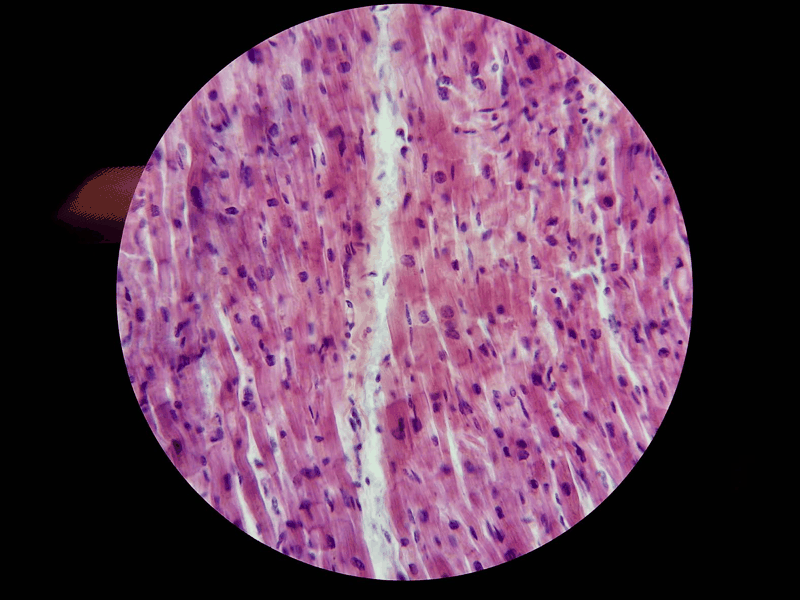
\includegraphics[width =
0.7\linewidth]
{biology-assets/animal-histology-cardiac.png}
\end{figure}
Cardiac muscle in longitudinal section, H\&E,
40x (practical 5): branched cells with
central nuclei and intercalated discs,
divided by a band of connective tissue.

\begin{figure}[ht]
\centering
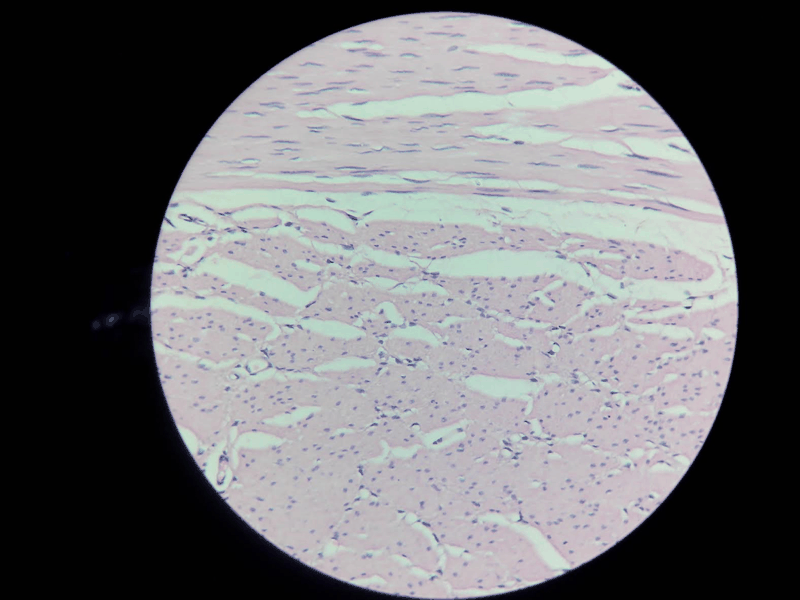
\includegraphics[width =
0.7\linewidth]
{biology-assets/animal-histology-smooth.png}
\end{figure}
Smooth muscle, H\&E, 40x (practical 5): one
layer cut lengthwise, with elongated nuclei,
and one cut across, separated by connective
tissue with a small blood vessel.

\begin{figure}[ht]
\centering
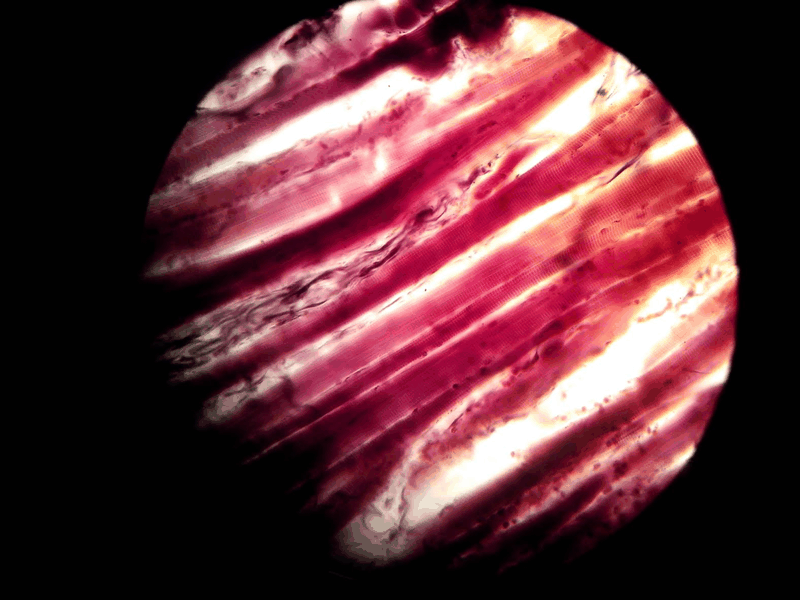
\includegraphics[width =
0.7\linewidth]
{biology-assets/animal-histology-skelet.png}
\end{figure}
Skeletal muscle of guinea-pig tongue, silver
technique, 40x (practical 5): striated fibres
in longitudinal section with peripheral
nuclei; Daniel's deck labels the A, I and H
bands and a nerve fascicle.

\section{Nervous tissue}
\label{section-nervous}

Nervous tissue consists of neurons and glial
cells; instead of connective tissue it has a
neuropil of interwoven cell processes
\cite[Chapter 12]{ross2011histology}. Neurons
are multipolar (most motor and association
neurons; Purkinje and pyramidal cells),
bipolar (retina, olfactory epithelium) or
pseudounipolar (sensory ganglia);
functionally they are sensory, motor or
interneurons. Their large euchromatic nuclei
and abundant rough endoplasmic reticulum
(Nissl bodies) reflect intense protein
synthesis.

\begin{center}
\begin{tabular}{ll}
Glial cell & Role \\
\hline
Oligodendrocyte & CNS myelin, one cell \\
& for many axons \\
Schwann cell & PNS myelin \\
Astrocyte & perivascular feet; \\
& K$^+$ buffering \\
Microglia & phagocytes \\
Ependymal cell & lines ventricles \\
& and central canal \\
Satellite cell & surrounds neurons \\
& in ganglia \\
M\"uller cell & retinal glia \\
\end{tabular}
\end{center}

Protoplasmic astrocytes are found in grey
matter and fibrous astrocytes in white
matter. The blood--brain barrier is formed by
the tight junctions of the capillary
endothelium, with astrocyte end-feet covering
the vessels. The brain and cord are wrapped
in three meninges (dura, arachnoid, pia), and
the choroid plexuses secrete the
cerebrospinal fluid \cite[Chapter
12]{ross2011histology}.

\textbf{Organization.} The neural tube forms
from an ectodermal groove; radial glia guide
migrating neurons, and its anterior end
swells into the prosencephalon (telencephalon
and diencephalon), mesencephalon and
rhombencephalon (metencephalon and
myelencephalon). In the spinal cord the grey
matter is central, with motor neurons in the
ventral horns, while the sensory neurons are
pseudounipolar cells in the dorsal root
ganglia. In the cerebrum and cerebellum the
grey matter forms an outer cortex: six layers
in the cerebral neocortex, three (molecular,
Purkinje and granular) in the cerebellum. A
nerve has endoneurium around each fibre,
perineurium around each fascicle and
epineurium around the whole. Sensory ganglia
have pseudounipolar neurons, autonomic
ganglia multipolar ones, each surrounded by
satellite cells and enclosed in a connective
tissue capsule.

The practical slides were a spinal ganglion
(pseudounipolar neurons and satellite cells),
cerebellum (Purkinje cells), cerebral cortex
(pyramidal cells), spinal cord (multipolar
motor neurons and ependyma), and fibrous
astrocytes and microglia shown by silver
impregnation. (The lab manual calls Purkinje
cells bipolar; they are multipolar.)

\section{Receptors and sense organs}
\label{section-senses}

Receptors are classified by location
(exteroceptors, interoceptors,
proprioceptors), by the stimulus (mechanical,
chemical, light, temperature), and by
structure: free nerve endings, encapsulated
endings, and secondary receptor cells,
modified epithelial cells innervated by a
neuron.

\textbf{Skin and muscle.} Free endings sense
temperature and pain; Merkel cells and
Meissner's corpuscles in the dermal papillae
sense light touch; Pacinian corpuscles in the
deep dermis and hypodermis sense pressure and
vibration; Ruffini endings sense stretch
\cite[Chapter 15]{ross2011histology}. Birds
have Herbst corpuscles, similar to Pacinian
corpuscles, in the bill and skin
\cite[Chapter 9]{bacha2000veterinary}. The
neuromuscular spindle, with intrafusal fibres
whose nuclei crowd at the centre, measures
muscle stretch.

\textbf{Taste and smell.} Taste buds are
barrel-shaped groups of cells opening by a
taste pore. Of the lingual papillae, filiform
papillae have no taste buds; fungiform,
foliate and circumvallate papillae have them,
and serous glands empty into the trench
around each circumvallate papilla
\cite[Chapter 16]{ross2011histology}. Many
mammals have, besides the main olfactory
epithelium, a vomeronasal organ, an enclosed
pouch on each side of the nose that detects
pheromones \cite[Chapter 14]{hill2012animal}.

\textbf{Hair cells and the lateral line.}
Hair cells are the mechanoreceptors of the
acoustico-lateralis system: vestibular
organs, the lateral line of fishes and
amphibians, and the cochlea. Each bears a
bundle of stereocilia increasing in height
towards one side, where a true cilium, the
kinocilium, may stand. Bending the bundle
towards the kinocilium depolarizes the cell
and raises the firing rate of its afferent
fibre; bending it away hyperpolarizes it.
Hair cells also receive efferent synapses
\cite[Chapter 14]{hill2012animal}. In the
lateral line the hair cells and their
supporting cells form \emph{neuromasts}, with
the hair bundles embedded in a gelatinous
cupula, on the skin or in canals.

\textbf{Inner, middle and outer ear.} The
otic vesicle, an invagination of surface
ectoderm beside the hindbrain, sinks into the
mesenchyme and forms the membranous
labyrinth; in Daniel's outline it divides
into utricle and saccule, the semicircular
ducts grow from the utricle, a duct from the
saccule elongates into the cochlea, and the
surrounding mesenchyme becomes cartilage and
then bone. The middle ear cavity and auditory
tube come from the endoderm of the first
pharyngeal pouch, and the tympanic membrane
forms where the first pharyngeal groove meets
it, from all three germ layers; the malleus,
incus and stapes connect the tympanum to the
oval window \cite[Chapter
25]{ross2011histology}. In the vestibule, the
maculae of the utricle and saccule carry
otoliths and sense linear acceleration and
gravity; the cristae in the ampullae of the
semicircular ducts, under a gelatinous
cupula, sense angular acceleration. In the
cochlea, the cochlear duct (scala media,
filled with endolymph) lies between the scala
vestibuli and the scala tympani (filled with
perilymph); the organ of Corti rests on the
basilar membrane under the tectorial
membrane, its hair cells held by phalangeal
cells.

\textbf{Eye.} The optic vesicles grow out
from the diencephalon and fold into optic
cups, which induce the overlying ectoderm to
form the lens. The eye has a fibrous tunic
(sclera and cornea), a vascular tunic
(choroid, ciliary body with the smooth muscle
of accommodation, and iris) and the retina
\cite[Chapter 24]{ross2011histology}. The
retina has ten layers:

\begin{enumerate}
\item retinal pigment epithelium;
\item layer of rods and cones;
\item outer limiting membrane (apical ends of
M\"uller cells);
\item outer nuclear layer (nuclei of rods and
cones);
\item outer plexiform layer (synapses of
photoreceptors with bipolar and horizontal
cells);
\item inner nuclear layer (bipolar,
horizontal, amacrine and M\"uller cells);
\item inner plexiform layer (synapses of
bipolar, amacrine and ganglion cells);
\item ganglion cell layer;
\item layer of optic nerve fibres;
\item inner limiting membrane (basal lamina
of M\"uller cells).
\end{enumerate}

\section{Heart, vessels and mouth}
\label{section-heart-mouth}

\textbf{Heart.} The heart wall has three
layers \cite[Chapter 13]{ross2011histology}:
the endocardium (endothelium, subendothelial
connective tissue, and a subendocardial layer
carrying the Purkinje fibres of the
conducting system), the myocardium, and the
epicardium, a mesothelium over connective
tissue and fat (the visceral layer of the
pericardium). A fibrous skeleton of dense
connective tissue anchors the muscle and the
valves, which are connective tissue plates
covered by endocardium and tethered by
chordae tendineae to the papillary muscles.

\textbf{Vessels.} Arteries and veins have
three tunics: intima (endothelium and
subendothelial tissue), media (smooth muscle
and elastic tissue) and adventitia
(connective tissue with the vessels and
nerves of the wall). Elastic arteries such as
the aorta have a media of fenestrated elastic
lamellae with smooth muscle between them.
Muscular arteries have a thick media of
circularly arranged smooth muscle bounded by
an internal elastic lamina and, in larger
ones, an external elastic lamina. Arterioles
control the flow into capillary beds, and in
a \emph{portal system} a vessel carries blood
from one capillary bed to another. Lymphatic
capillaries begin blind and return tissue
fluid through lymph nodes to the blood
\cite[Chapter 13]{ross2011histology}.

\textbf{Oral cavity.} The oral mucosa is
masticatory (keratinized or parakeratinized,
on the gingiva and hard palate), lining
(non-keratinized, on lips, cheeks, floor and
soft palate) or specialized (the dorsum of
the tongue with its papillae) \cite[Chapter
16]{ross2011histology}. The tongue is a mass
of striated muscle running in three planes. A
tooth consists of enamel, the hardest tissue
of the body (96--98\% hydroxyapatite, made by
ameloblasts of ectodermal origin), dentin
(made by odontoblasts, whose processes remain
in the dentinal tubules), cementum on the
root, and the pulp of loose connective tissue
with vessels and nerves; the periodontal
ligament holds it in the alveolar bone. In
development, dentin is laid down first and
enamel on top of it. The major salivary
glands are the parotid (serous), the
submandibular (mixed, mostly serous) and the
sublingual (mixed, mostly mucous); their
secretory units drain through intercalated,
striated and excretory ducts.

\section{Urinary system}
\label{section-urinary}

\textbf{Kidney.} The cortex contains the
renal corpuscles and convoluted tubules (the
cortical labyrinth) and the medullary rays of
straight tubules; the medulla forms pyramids
whose apices, the papillae, open into the
minor calyces, which join into major calyces
and the renal pelvis; cortical tissue between
the pyramids forms the renal columns. A
\emph{lobe} is a pyramid with its covering
cortex; a \emph{lobule} is a medullary ray
with the nephrons draining into its
collecting duct \cite[Chapter
20]{ross2011histology}.

\textbf{Nephron.} The renal corpuscle is a
tuft of glomerular capillaries inside the
double-walled Bowman's capsule, with a
vascular pole (afferent and efferent
arterioles) and a urinary pole. The tubule
continues as proximal convoluted and straight
tubules, thin descending and ascending limbs,
distal straight tubule, distal convoluted
tubule and connecting tubule, ending in a
collecting duct that joins others into a
papillary duct. Cortical nephrons have short
loops; juxtamedullary nephrons have long
loops reaching deep into the medulla.

\textbf{Filtration barrier.} Plasma is
filtered through the fenestrated endothelium,
the thick glomerular basement membrane, and
the filtration slits between the
interdigitating pedicels of the podocytes,
bridged by a slit diaphragm containing
nephrin. Large and negatively charged
molecules such as albumin are held back.
Mesangial cells, enclosed by the basement
membrane among the capillaries, phagocytose
and support the tuft \cite[Chapter
20]{ross2011histology}.

\textbf{Making urine.} About 65\% of the
ultrafiltrate is reabsorbed in the proximal
tubule, a cuboidal epithelium with a brush
border and basal folds packed with
mitochondria: Na$^+$ is pumped out and water,
glucose, amino acids and small peptides
follow; filtered proteins are taken up by
endocytosis. The thin descending limb is
permeable to water, which leaves into the
hyperosmotic medullary interstitium; the
ascending limb is impermeable to water but
exports salt, so the fluid entering the
distal tubule is hyposmotic. The distal
tubule reabsorbs more Na$^+$ and secretes
K$^+$ and H$^+$. In the collecting duct,
principal (light) cells regulate water
reabsorption through aquaporins under
antidiuretic hormone, and intercalated (dark)
cells secrete H$^+$ or bicarbonate. The vasa
recta run in hairpin loops alongside the
loops of Henle and maintain the medullary
gradient by passive countercurrent exchange
\cite[Chapter 20]{ross2011histology}.

\textbf{Endocrine functions.} The
\emph{juxtaglomerular apparatus} at the
vascular pole comprises the macula densa
(crowded cells of the distal straight tubule
that sense the Na$^+$ concentration of the
tubular fluid), the juxtaglomerular cells
(modified smooth muscle cells of the afferent
arteriole containing renin granules) and the
extraglomerular mesangial cells. When Na$^+$
or blood pressure falls, renin is released;
it cleaves angiotensinogen to angiotensin I,
which is converted to angiotensin II, a
vasoconstrictor that also stimulates the
adrenal cortex to secrete aldosterone, which
raises Na$^+$ and water reabsorption. The
kidney also secretes erythropoietin, which
drives red cell production; Ross attributes
it to the endothelial cells of the
peritubular capillaries \cite[Chapter
20]{ross2011histology}.

\textbf{Excretory passages.} Calyces, pelvis,
ureter and bladder are lined by urothelium, a
transitional epithelium impermeable to water
and salts that flattens as the organ
distends, over a lamina propria, a muscularis
of interwoven smooth muscle bundles, and an
adventitia. The male urethra is lined by
urothelium in its prostatic part, by
stratified or pseudostratified columnar
epithelium in its membranous and spongy
parts, and by stratified squamous epithelium
near its opening; the female urethra is lined
mainly by stratified squamous epithelium
\cite[Chapter 20]{ross2011histology}.

\section{Reproductive systems}
\label{section-reproductive}

\textbf{Testis.} The testis is enclosed by
the tunica vaginalis (a mesothelium), the
dense tunica albuginea and the vascular
tunica vasculosa \cite[Chapter
22]{ross2011histology}. The seminiferous
tubules have a stratified epithelium of
spermatogenic cells and Sertoli cells,
surrounded by contractile peritubular myoid
cells; Leydig cells lie in the interstitium
between the tubules.

\begin{itemize}
\item \emph{Spermatogenesis}: type A dark
spermatogonia (reserve stem cells) give type
A pale spermatogonia, which give type B
spermatogonia; these become primary
spermatocytes, the largest cells, which
complete meiosis I to give secondary
spermatocytes, short-lived and rarely seen,
which complete meiosis II to give spermatids.
\item \emph{Spermiogenesis}: the spermatid
condenses its nucleus, forms an acrosome from
the Golgi apparatus, grows a flagellum,
gathers its mitochondria into the middle
piece and sheds the excess cytoplasm.
\item \emph{Sertoli cells}, with a pale oval
nucleus and a large nucleolus, support the
germ cells; their occluding junctions form
the blood--testis barrier. They secrete
androgen-binding protein (which concentrates
testosterone in the tubule), inhibin (which
feeds back on FSH secretion) and, in the
fetus, anti-M\"ullerian hormone.
\item \emph{Leydig cells}, large and
eosinophilic with abundant smooth endoplasmic
reticulum and lipid droplets (and Reinke
crystals in humans), make testosterone under
LH.
\end{itemize}

The sperm pass from the seminiferous tubules
through the straight tubules (lined only by
Sertoli cells) to the rete testis in the
mediastinum, then through the efferent
ductules (ciliated and absorptive cells) to
the epididymis, a coiled duct lined by
pseudostratified epithelium with stereocilia,
and on to the ductus deferens with its thick
three-layered muscularis. The accessory
glands are the seminal vesicles, the prostate
and the bulbourethral glands; the penis has
two dorsal corpora cavernosa and a ventral
corpus spongiosum around the urethra
\cite[Chapter 22]{ross2011histology}.

\textbf{Ovary.} The ovary is covered by the
germinal epithelium, a simple cuboidal or
squamous mesothelium (not germinal), over a
tunica albuginea; the cortex holds the
follicles and the medulla vessels and nerves
\cite[Chapter 23]{ross2011histology}. A
primordial follicle is a primary oocyte,
arrested in prophase of meiosis I, inside one
layer of flat follicle cells. In a primary
follicle the follicle cells become cuboidal
granulosa cells and the zona pellucida
appears; in a secondary follicle a
fluid-filled antrum forms and the stroma
around it differentiates into the theca
interna and externa. Theca interna cells make
androgens, which the granulosa cells convert
into estrogens. Just before ovulation the
oocyte completes meiosis I and gives off the
first polar body; meiosis II is completed
only at fertilization. After ovulation the
follicle becomes the corpus luteum, of large
granulosa lutein cells and small theca lutein
cells, which secretes progesterone and
estrogens; without pregnancy it degenerates
into a corpus albicans. Most follicles never
mature and degenerate (atresia).

\textbf{Genital tract.} The oviduct
(infundibulum with fimbriae, ampulla, isthmus
and intramural part) is lined by a simple
columnar epithelium of ciliated and secretory
cells over a highly folded mucosa, with a
muscularis and a serosa. The uterine wall
consists of endometrium (simple columnar
epithelium with simple tubular glands),
myometrium and perimetrium. The endometrium
has a functional layer, shed at menstruation,
and a basal layer from which it regenerates;
it is supplied by spiral arteries and passes
through menstrual, proliferative and
secretory phases. The cervical mucosa, with
large branched glands, is not shed. The
vagina is lined by non-keratinized stratified
squamous epithelium, has no glands and is
lubricated by cervical mucus. The mammary
gland is a compound tubuloalveolar gland of
lobes separated by connective tissue and fat;
its lipid is secreted in apocrine fashion and
its proteins by merocrine secretion
\cite[Chapter 23]{ross2011histology}.

\section{Endocrine glands in evolution}
\label{section-endocrine}

The endocrine exam showed four micrographs
and asked, for each gland, what it is, in
which vertebrates, what it does, and how its
organization changed in evolution. Daniel's
answers covered an amphibian adrenal, a
parathyroid inside the thymus, a reptile
pineal and a testis (described above).
Endocrine glands are richly vascularized
cords or follicles of secretory cells without
ducts, and their output is usually regulated
by negative feedback.

\textbf{Adrenal gland.} In mammals a cortex
of steroid-secreting cells surrounds a
medulla of chromaffin cells \cite[Chapter
21]{ross2011histology}. The cortex is
mesodermal and has three zones: glomerulosa
(mineralocorticoids such as aldosterone),
fasciculata (glucocorticoids such as
cortisol) and reticularis (weak androgens).
The chromaffin cells derive from the neural
crest; innervated by preganglionic
sympathetic fibres, they act as
postganglionic neurons that secrete
epinephrine and norepinephrine into the
blood. In culture they grow axon-like
processes, which glucocorticoids from the
cortex suppress, so the cortex shapes the
medulla. In the other vertebrates the two
tissues are called interrenal and chromaffin,
and the trend is from separation to intimate
association \cite[Chapter
13]{andrew1959comparative}:

\begin{center}
\begin{tabular}{ll}
Group & Interrenal and \\
& chromaffin tissue \\
\hline
Cyclostomes & separate: interrenal \\
& bodies along veins, \\
& chromaffin strips \\
Elasmobranchs & separate: interrenal \\
& body; chromaffin \\
& paraganglia \\
Bony fishes & mingled \\
Amphibians & paired glands on \\
& the kidneys; mixed \\
& cords and islands \\
Reptiles & irregular mixture \\
Birds & intertwined cords \\
Mammals & cortex around \\
& medulla \\
\end{tabular}
\end{center}

Birds do not have a cortex and a medulla:
their cortical cords are interwoven with
masses of chromaffin cells throughout the
gland \cite[Chapter 16]{bacha2000veterinary}.
Daniel's amphibian slide showed the
chromaffin cells in cords between sinusoids,
with sympathetic neurons, and no
steroidogenic tissue in the field.

\textbf{Parathyroid gland.} The parenchyma is
cords of principal (chief) cells, which
secrete parathyroid hormone (PTH), and larger
acidophilic oxyphil cells, among capillaries
\cite[Chapter 21]{ross2011histology}. PTH
raises blood calcium by promoting bone
resorption, calcium reabsorption in the
kidney and the activation of vitamin D, while
it increases the renal excretion of
phosphate; calcitonin from the thyroid's
parafollicular cells opposes it. Fishes
appear to have no parathyroids; in amphibians
they are minute bodies near the jugular vein;
in birds accessory parathyroid tissue occurs
in the thymus; most mammals have two pairs,
but rats and mice usually one, and in several
mammals one pair lies inside the thyroid
\cite[Chapter 13]{andrew1959comparative}.
Daniel identified his parathyroid by its
compact vascularized cords without lobules or
colloid, and the surrounding tissue as thymus
by its densely packed lymphocytes.

\textbf{Pineal gland.} The pineal develops
from neuroectoderm of the roof of the
diencephalon and remains attached to the
brain by a stalk \cite[Chapter
21]{ross2011histology}. In mammals it is a
solid gland of pinealocytes in clumps and
cords, with interstitial glial cells
resembling astrocytes (about 5\% of the
cells) and, in humans, calcified concretions
(corpora arenacea, brain sand) that increase
with age. It secretes melatonin at night,
under control of the suprachiasmatic nucleus.
In fishes and amphibians the pineal is
hollow; in lizards and turtles it is hollow
with folded walls, in snakes solid, and in
birds hollow, chambered or solid according to
the group; in the tuatara \emph{Sphenodon} a
parietal ``third eye'' is especially
prominent \cite[Chapter
13]{andrew1959comparative}. Unlike the
mammalian gland, the pineal of many
non-mammalian vertebrates is itself
light-sensitive and may be an independent
circadian clock \cite[Chapter
15]{hill2012animal}. Melatonin lightens the
skin of amphibians and lampreys
\cite[Appendix K]{hill2012animal}. Daniel's
answer summed up the trend as a shift from a
hollow, photoreceptive organ to a solid gland
whose cells are mainly secretory.

\textbf{Gonads.} Daniel's talk on the
endocrine cells of the reproductive organs
covered the Leydig and Sertoli cells, the
theca cells, the lutein cells of the corpus
luteum, and the interstitial cells left by
atretic follicles, which also secrete
steroids (see
Section~\ref{section-reproductive}).

\begin{figure}[ht]
\centering
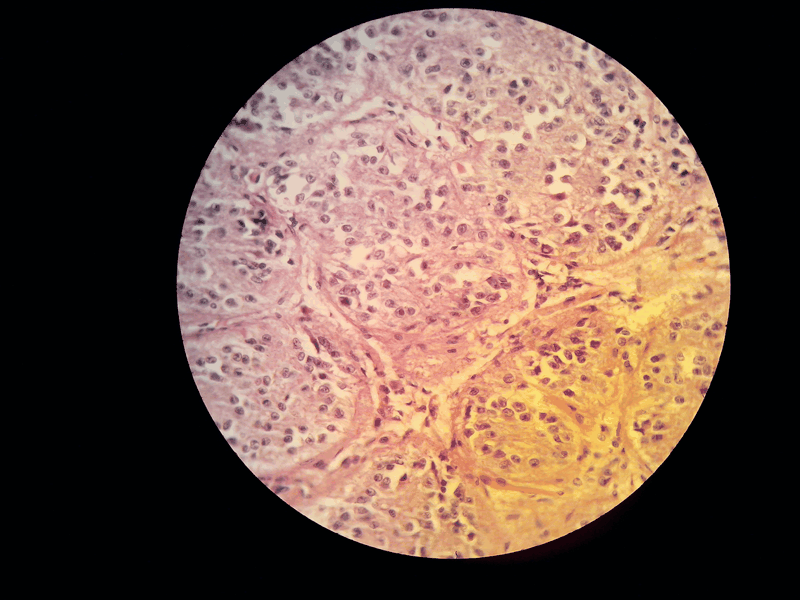
\includegraphics[width =
0.7\linewidth]
{biology-assets/animal-histology-pineal.png}
\end{figure}
Mammalian pineal gland, H\&E, 40x:
pinealocytes in clumps (parenchymal lobules)
separated by thin connective tissue septa.

\begin{figure}[ht]
\centering
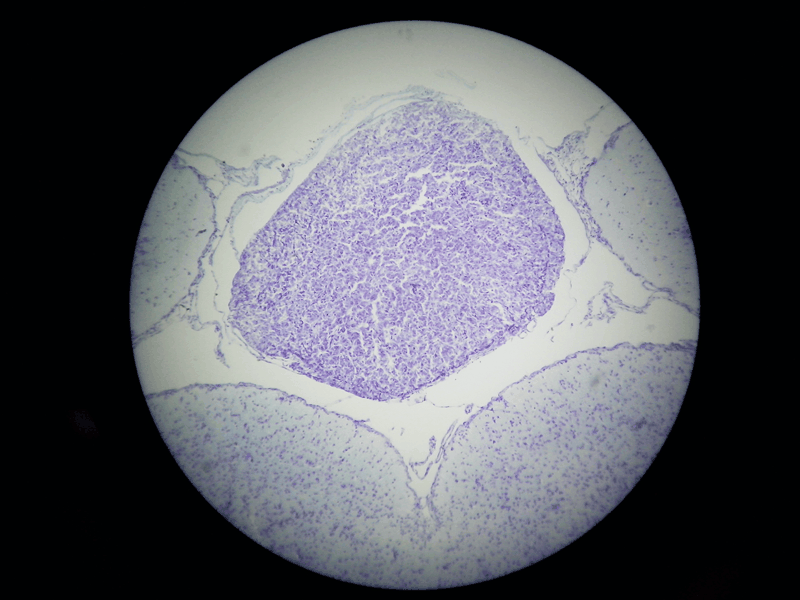
\includegraphics[width =
0.7\linewidth]
{biology-assets/animal-histology-pinrat.png}
\end{figure}
Rat pineal gland, 10x (stain not recorded):
the gland in place among the brain tissue,
wrapped in meninges.

\begin{figure}[ht]
\centering
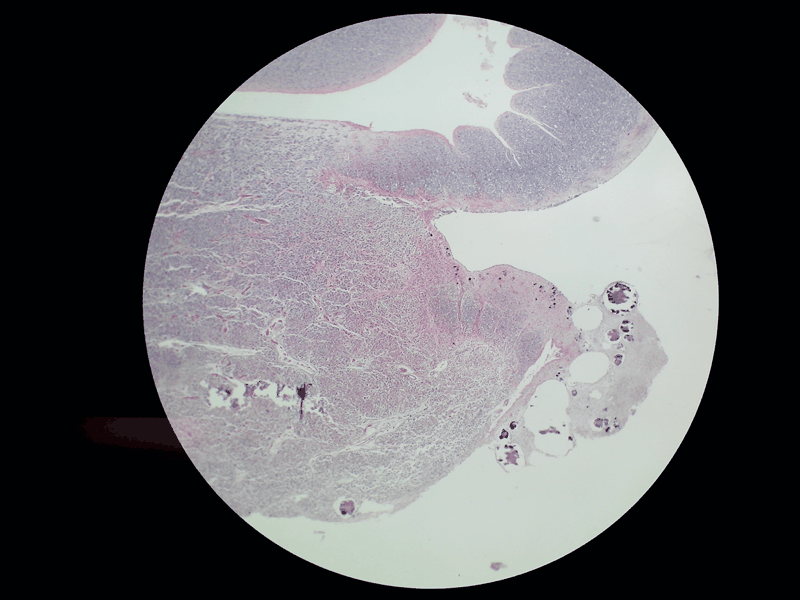
\includegraphics[width =
0.7\linewidth]
{biology-assets/animal-histology-pinhum.png}
\end{figure}
Human pineal gland, H\&E, 5x: the dark purple
bodies at the right and lower left are
calcified concretions (brain sand); blood
vessels run through the parenchyma.

\begin{figure}[ht]
\centering
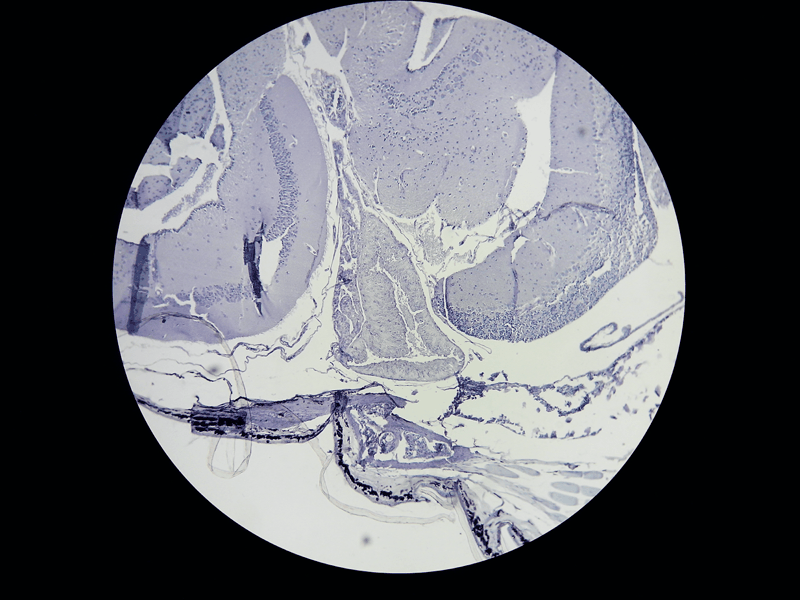
\includegraphics[width =
0.7\linewidth]
{biology-assets/animal-histology-pinrep.png}
\end{figure}
Reptile pineal gland (species not recorded),
PAS, 10x: the gland, with hollow spaces
absent from the mammalian pineal, lies
between the brain and the skull.

\begin{figure}[ht]
\centering
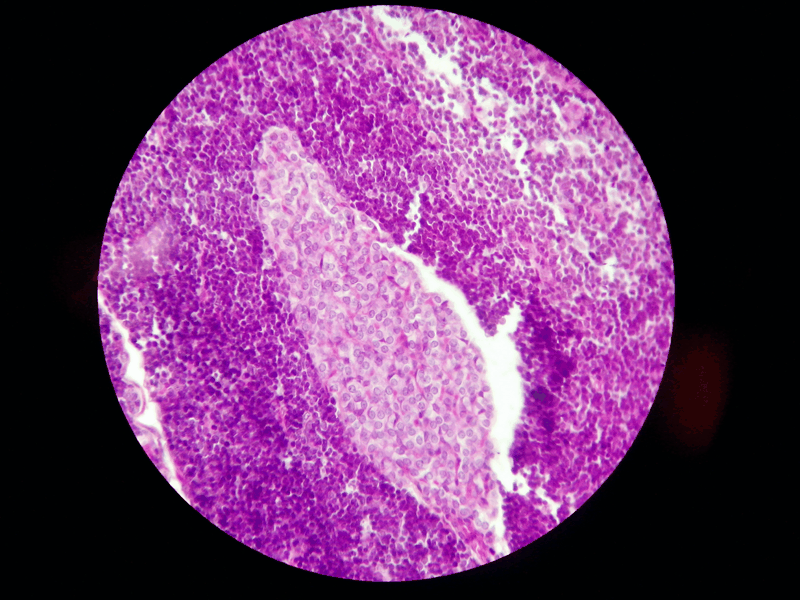
\includegraphics[width =
0.7\linewidth]
{biology-assets/animal-histology-parathy.png}
\end{figure}
Parathyroid tissue inside the thymus, H\&E,
40x: a pale island of chief cells in cords,
with blood vessels, surrounded by densely
packed thymic lymphocytes (the micrograph of
the exam question).

\begin{figure}[ht]
\centering
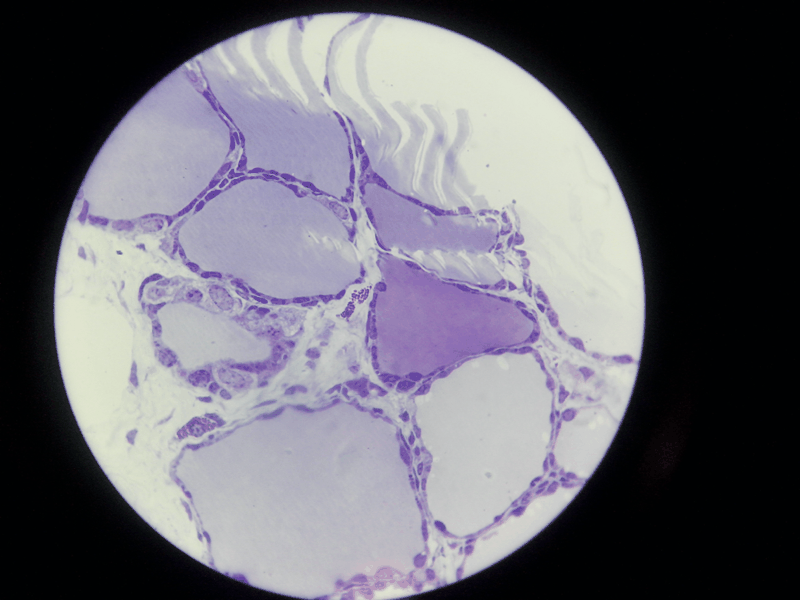
\includegraphics[width =
0.7\linewidth]
{biology-assets/animal-histology-thyroid.png}
\end{figure}
Mammalian thyroid gland, 40x (stain not
recorded): follicles of flattened follicular
cells around colloid; Daniel's deck marks a
parafollicular cell and mast cells in the
connective tissue between follicles.

\begin{figure}[ht]
\centering
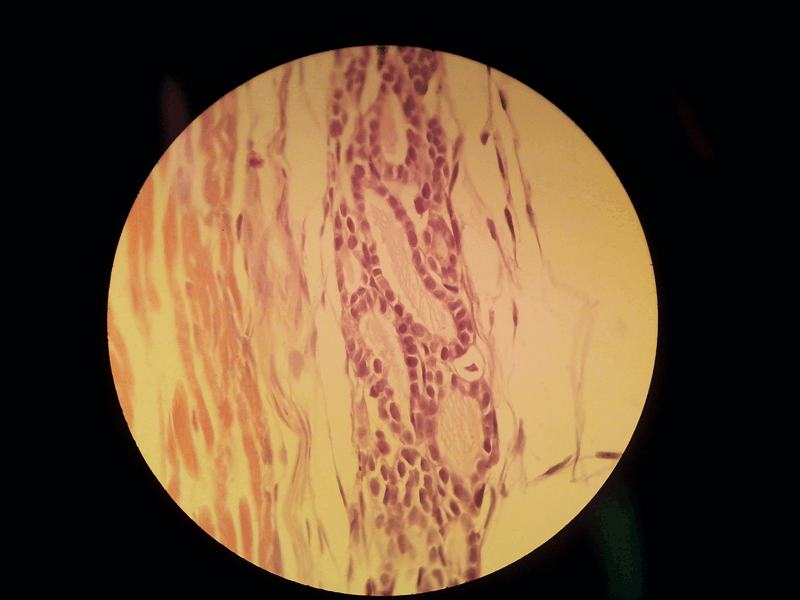
\includegraphics[width =
0.7\linewidth]
{biology-assets/animal-histology-thyaxo.png}
\end{figure}
Thyroid of an axolotl, H\&E, 10x: small
follicles with colloid and secretory cells
among connective tissue.

\section{Natural killer cells}
\label{section-nk}

Natural killer (NK) cells are the third kind
of lymphocyte, besides T and B cells. They
develop from the same precursor in the bone
marrow but do not mature in the thymus. They
are large granular lymphocytes (about 15
$\mu$m, kidney-shaped nucleus, azurophilic
granules) and are recognized by the markers
CD16, CD56 and CD94 \cite[Chapters 10 and
14]{ross2011histology} and by the absence of
the T cell marker CD3 \cite{cooper2001nk}.
Estimates of their share of blood lymphocytes
range from 5--10\% \cite[Chapter
14]{ross2011histology} to about 15\%
\cite{cooper2001nk}.

\textbf{Killing.} NK cells kill
virus-infected and tumour cells without prior
sensitization, releasing perforin and
granzymes that drive the target into
apoptosis, as cytotoxic T cells do
\cite[Chapter 14]{ross2011histology}. Their
targets are chosen by a balance of activating
and inhibitory receptors. The inhibitory
receptors (KIRs and CD94--NKG2A in humans)
recognize MHC class I molecules, so a cell
that has lost them, as many virus-infected
and tumour cells do, is attacked: the
``missing self'' principle
\cite{munz2005dendritic}. NK cells also kill
antibody-coated cells by antibody-dependent
cellular cytotoxicity, binding the Fc portion
of IgG through CD16 \cite{cooper2001nk}.

\textbf{Regulation.} Human NK cells form two
subsets: about 90\% are
CD56$^{\mathrm{dim}}$CD16$^{\mathrm{bright}}$
and highly cytotoxic, and about 10\%
CD56$^{\mathrm{bright}}$, with little
cytotoxicity but abundant cytokine production
\cite{cooper2001nk}. Activated NK cells
secrete interferon $\gamma$, TNF-$\alpha$ and
other cytokines and chemokines, and they
promote the maturation of dendritic cells,
which then prime T cells: a bridge between
innate and adaptive immunity
\cite{munz2005dendritic}.

Daniel and his lab partner wrote the essay as
a mock presidential campaign for the NK cell,
praising its speed, its independence from
antigen presentation, its cytokines, its help
to dendritic cells, its reported memory-like
behaviour, and NK-like cells described in
echinoderms and annelids as a sign of ancient
origin. The textbook picture corrects one
point of the essay: NK cells do not ignore
MHC molecules but use MHC class I as the
signal to spare a cell.

\section{The semicircular canals}
\label{section-canals}

Daniel's final paper, \emph{La importancia de
saber d\'onde est\'a tu cabeza} (``Why it
matters to know where your head is''), asked
how the three semicircular canals of each ear
are oriented and why.

\textbf{Background.} Each semicircular duct
(inside its bony canal) is filled with
endolymph. Its ampulla holds a crista whose
hair cells project into a gelatinous cupula;
when the head rotates, the endolymph lags,
deflects the cupula and excites or inhibits
the hair cells according to the direction of
bending. Since the fluid moves relative to
the head only when the rotation changes, the
canals sense angular acceleration. Each canal
responds to rotation about one axis, in two
senses, so at least three non-coplanar canals
are needed to reconstruct an arbitrary
rotation in three-dimensional space; the
canals of each ear are at approximately right
angles \cite[Chapter 14]{hill2012animal}.

\textbf{Data.} The paper compiled the
measured angles between canal planes from
published studies (Blanks and colleagues for
monkeys, rat and frog; Della Santina and
colleagues for humans, by CT reconstruction;
Calabrese and Hullar for two mouse strains;
Hullar and Williams for the chinchilla;
Dickman for the pigeon). Two kinds of angle
were tabulated: between the three canals of
one ear, and between the canals that should
be parallel across the head, namely the two
lateral canals, and each anterior canal with
the opposite posterior one, which are excited
and inhibited together by the same rotation.

\textbf{Results and conclusion.} The
ipsilateral angles cluster near 90 degrees:
for humans 90.6, 90.4 and 94.0 degrees on
average. The exceptions were the pigeon,
whose angles all fall below 90 degrees (about
76 to 87), and the chinchilla, where they
range from about 76 to 103 degrees. The
supposedly parallel pairs are not parallel:
most differ by roughly 8 to 20 degrees,
typically around 15 (reported as 160 to 172
degrees by studies that measure the angle the
other way round), while the frog's pairs, and
the lateral canals of the rhesus monkey and
the pigeon, are within a few degrees of
parallel. Daniel concluded that
near-orthogonality is a widespread property
tied to how the brain decodes rotation: three
mutually perpendicular planes make the three
signals as independent as possible.

\textbf{Epilogue.} The axes of maximal
sensitivity of the canal afferents, measured
physiologically, differ by a few degrees from
the anatomical canal axes, though they too
are roughly orthogonal. Following Rabbitt's
1999 model of endolymph flow, the paper noted
that a rotation about one canal's sensitivity
axis still excites the other two nerves, and
that the three rotation axes that each excite
only one nerve are, according to the model,
not orthogonal, which leaves open why the
canals are arranged as they are.

\bibliography{my}
\bibliographystyle{amsalpha}

\end{document}
